\section{Effektforstærker}
\begin{frame}{Effektforstærker}
Krav opsat til effektforstærkeren

\scriptsize{\begin{table}[h]
\centering
\begin{tabular}{l|r}
\hline\hline
Område & Krav \\
\hline\hline
Klasse & AB \\[4pt]
Nyttevirkning & \> 25 \%  \\[4pt]
Forvrængning & \< 0,5 \% \\[4pt]
Udgangseffekt & \> 20 W ved 2 V input \\[4pt]
Frekvensgang & \< 0,375 dB ved 20 Hz - 20 kHz, ref. 1 kHz \\
& \< 0,75 dB fra 20 Hz til 63 Hz \\
& \< 0,75 dB fra 12,5 kHz til 20 kHz \\[4pt]
Belastningsimpedans & 8 \ohm \\[4pt]
Udgangssignaltype & Mono \\[4pt]
Kortslutningsstrøm (peak) & 3 A \\
\hline\hline
\end{tabular}
\end{table}}

\end{frame}


\begin{frame}{Opbygning}

 LIN 3-stage topologi

\begin{itemize}
\item Differensforstærker 
\item Spændingsforstærker
\item Strømforstærker 
\item Tilbagekobling
\end{itemize}

\begin{figure}[h]
\centering
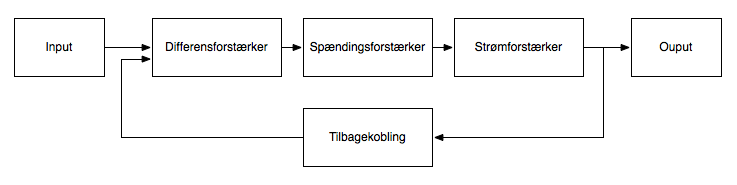
\includegraphics[scale=0.35]{images/blokdiagram-effektforstaerker.png}
\end{figure}

\end{frame}

%\begin{frame}{Termiske Forhold}
%\begin{itemize}
%\item 110 mm Køleplade
%\end{itemize}
%\begin{figure}[h]
%\centering
%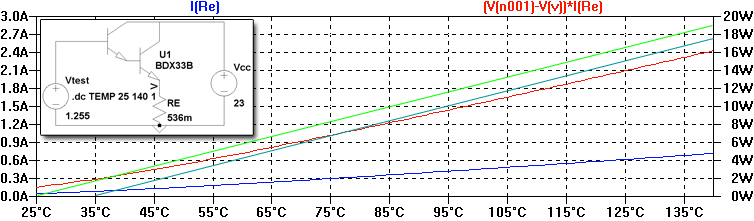
\includegraphics[width=\textwidth]{images/term-runaway.png}
%\end{figure}
%\begin{itemize}
%\item 150 mm Køleplade 
%\end{itemize}
%\begin{figure}[h]
%\centering
%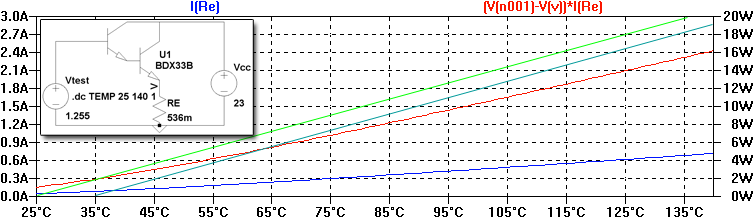
\includegraphics[width=\textwidth]{images/term-runaway1.png}
%\end{figure}
%\end{frame}


\begin{frame}{Stabilitet}

\begin{itemize}
\item Ukorrigeret
\end{itemize}
\begin{figure}[h]
\centering
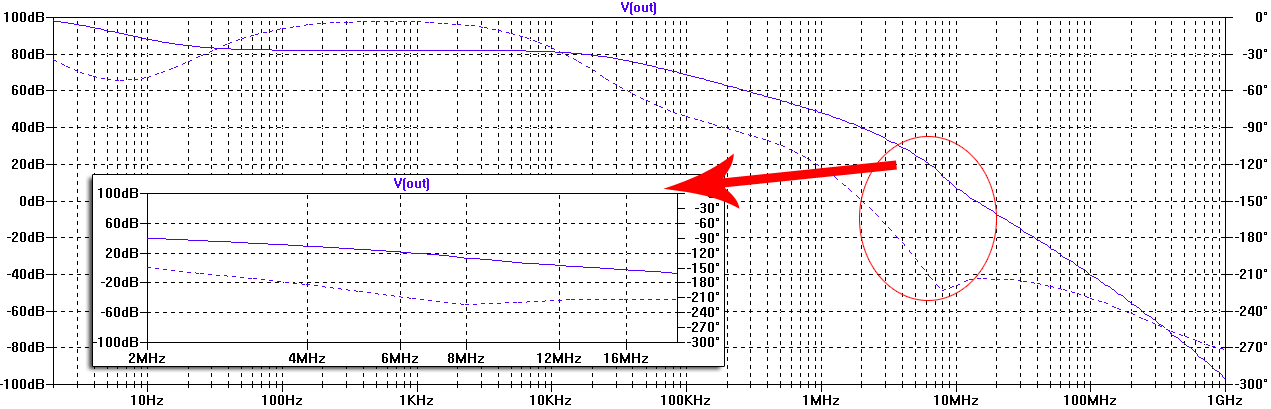
\includegraphics[width=\textwidth]{images/stabilitet-udenc-graf.png}
\end{figure}

\begin{itemize}
\item Korrigeret
\end{itemize}
\begin{figure}[h]
\centering
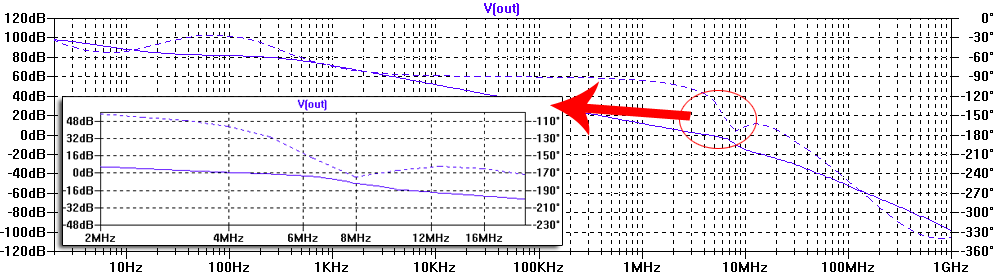
\includegraphics[width=\textwidth]{images/stabilitet-medc-graf.png}
\end{figure}

\end{frame}


\begin{frame}{Frekvensgang}

\begin{figure}[h]
\centering
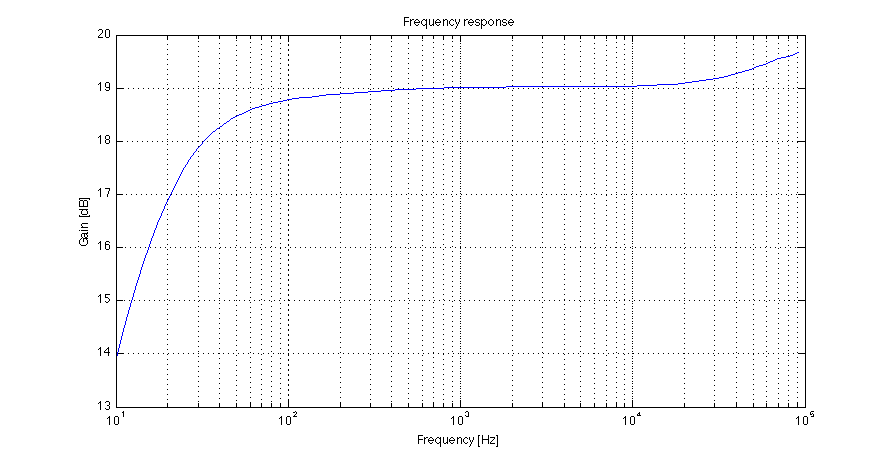
\includegraphics[width=\textwidth]{images/2V-45mA-uden-modstand-frek.png}
\end{figure}

\scriptsize{\begin{table}[h]
\centering
\begin{tabular}{l|r|r}
\hline\hline
Område & Krav & Status \\
\hline\hline
Frekvensgang & \< 0,375 dB ved 20 Hz - 20 kHz, ref. 1 kHz & $\mathcal{X}$ \\
& \< 0,75 dB fra 20 Hz til 63 Hz & $\mathcal{X}$ \\
& \< 0,75 dB fra 12,5 kHz til 20 kHz & \checkmark \\[4pt]
\hline\hline
\end{tabular}
\end{table}}


\end{frame}

\begin{frame}{THD}

\begin{figure}[h]
\centering
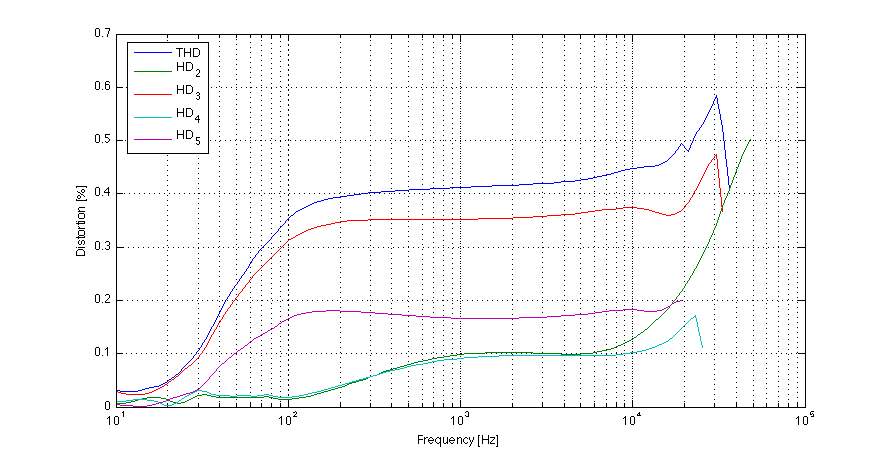
\includegraphics[width=\textwidth]{images/2V-45mA-uden-modstand-thd.png}
\end{figure}

\scriptsize{\begin{table}[h]
\centering
\begin{tabular}{l|r|r}
\hline\hline
Område & Krav & Status \\
\hline\hline
Forvrængning & \< 0,5 \% & \checkmark \\[4pt]
\hline\hline
\end{tabular}
\end{table}}

\end{frame}


\begin{frame}{Accepttest}

\scriptsize{\begin{table}[h]
\centering
\begin{tabular}{l|r|r}
\hline\hline
Område & Krav \\
\hline\hline
Klasse & AB & \checkmark \\[4pt]
Nyttevirkning & \> 25 \%  & \checkmark \\[4pt]
Forvrængning & \< 0,5 \% & \checkmark \\[4pt]
Udgangseffekt & \> 20 W ved 2 V input & $\mathcal{X}$ \\[4pt]
Frekvensgang & \< 0,375 dB ved 20 Hz - 20 kHz, ref. 1 kHz & $\mathcal{X}$ \\
& \< 0,75 dB fra 20 Hz til 63 Hz & $\mathcal{X}$ \\
& \< 0,75 dB fra 12,5 kHz til 20 kHz & \checkmark \\[4pt]
Belastningsimpedans & 8 \ohm & \checkmark \\[4pt]
Udgangssignaltype & Mono & \checkmark \\[4pt]
Kortslutningsstrøm (peak) & 3 A & $\mathcal{X}$ \\
\hline\hline
\end{tabular}
\end{table}}

\end{frame}

